% This file was converted to LaTeX by Writer2LaTeX ver. 1.4
% see http://writer2latex.sourceforge.net for more info
\documentclass[a4paper]{article}
\usepackage[utf8]{inputenc}
\usepackage[T1]{fontenc}
\usepackage[ngerman]{babel}
\usepackage{amsmath}
\usepackage{amssymb,amsfonts,textcomp}
\usepackage{color}
\usepackage{array}
\usepackage{hhline}
\usepackage{hyperref}
\hypersetup{pdftex, colorlinks=true, linkcolor=blue, citecolor=blue, filecolor=blue, urlcolor=blue, pdftitle=}
\usepackage[pdftex]{graphicx}
% footnotes configuration
\makeatletter
\renewcommand\thefootnote{\arabic{footnote}}
\makeatother
% Text styles
\newcommand\textstyleFootnoteSymbol[1]{#1}
\newcommand\textstyleAbsatzStandardschriftart[1]{#1}
% Outline numbering
\setcounter{secnumdepth}{0}
% List styles
\newcommand\liststyleLi{%
\renewcommand\labelitemi{•}
\renewcommand\labelitemii{◦}
\renewcommand\labelitemiii{${\blacksquare}$}
\renewcommand\labelitemiv{•}
}
\newcommand\liststyleLii{%
\renewcommand\labelitemi{•}
\renewcommand\labelitemii{◦}
\renewcommand\labelitemiii{${\blacksquare}$}
\renewcommand\labelitemiv{•}
}
\newcommand\liststyleLiii{%
\renewcommand\labelitemi{•}
\renewcommand\labelitemii{◦}
\renewcommand\labelitemiii{${\blacksquare}$}
\renewcommand\labelitemiv{•}
}
% Page layout (geometry)
\setlength\voffset{-1in}
\setlength\hoffset{-1in}
\setlength\topmargin{2cm}
\setlength\oddsidemargin{3.5cm}
\setlength\textheight{22.706001cm}
\setlength\textwidth{15.500999cm}
\setlength\footskip{1.497cm}
\setlength\headheight{0.998cm}
\setlength\headsep{0.499cm}
% Footnote rule
\setlength{\skip\footins}{0.119cm}
\renewcommand\footnoterule{\vspace*{-0.018cm}\setlength\leftskip{0pt}\setlength\rightskip{0pt plus 1fil}\noindent\textcolor{black}{\rule{0.25\columnwidth}{0.018cm}}\vspace*{0.101cm}}
% Pages styles
\makeatletter
\newcommand\ps@Standard{
  \renewcommand\@oddhead{\sffamily INM - Potentielle Neuordnung des Informationsmanagements\hfill 27.05.15}
  \renewcommand\@evenhead{\@oddhead}
  \renewcommand\@oddfoot{\sffamily INM – SoSe 2015\hfill \hfill \thepage{} / ?}
  \renewcommand\@evenfoot{\@oddfoot}
  \renewcommand\thepage{\arabic{page}}
}
\makeatother
\pagestyle{Standard}
\title{}
\begin{document}
\section{1 Marketing}
{\sffamily
Das Marketing hat neben dem typischen Aufgabenbereich der Außenrepräsentation durch die Besonderheiten einer Hochschule
auch einen Aufgabenbereich der Innenrepräsentation. Im folgenden werden diese Bereiche getrennt betrachtet.}

\subsection{1.1 Externes Hochschulmarketing}
{\sffamily
Das externe Marketing der Hochschule bezieht sich auf die klassischen Marketingaufgaben, das Produkt und die Marke
vorteilhaft darzustellen. Im Falle einer Hochschule ist dies die attraktive Darstellung gegenüber zukünftige
Studierenden, Forschungsinteressierten und Geldgebern.}

\subsection{1.1.1 Webseite}
{\sffamily
Zentrales Element bleibt die Hochschulwebseite, die mit aktuellen, offenen Möglichkeiten von HTML 5, CSS 3 und
JavaScript den Funktionsumfang einer App erreichen kann, ohne auf spezielle oder spezifische Spezialtechnologien zu
setzen. Besonders sei an dieser Stelle die Möglichkeit genannt, mittels CSS Größen und Darstellungsmöglichkeiten von
Endgeräten unabhängig von konkreten Betriebssystemen und Hardwareplattformen abzudecken.}

{\sffamily
Dies ist vor dem Hintergrund wichtig, dass beispielsweise eine native App für iPhones zwingend durch den Appstore der
Firma Apple installiert werden muss, dessen Nutzungsbedingungen sich für die Hochschule in Form von Kosten oder
Inhaltseinschränkungen zu Ungunsten der Hochschule verändern könnten. Mit einer nativen App lässt sich trotzdem nur ein
beschränkter Nutzerkreis ansprechen. Sollen mehrere Apps für verschiedene Plattformen gepflegt werden, so ist dies mit
zusätzlichen Aufwand verbunden.}

{\sffamily
Eine Neuauflage der Hochschulwebseite mit aktuellen Möglichkeiten und per CSS an verschiedene Darstellungsgrößen
angepasst erreicht dagegen jedes internetfähige Gerät mit Browser. Sollte ein neuer Formfaktor wichtig werden, zum
Beispiel der einer Smartwatch, so lässt sich dies über eine Erweiterung des Stylesheets erreichen, ohne eine komplette
Neuentwicklung in Auftrag zu geben.}

\subsection{1.1.2 Soziale Netzwerke}
{\sffamily
Soziale Netzwerke wie facebook oder twitter sind kritisch zu bewerten. Auftritte auf diesen Plattformen können nicht
alleine stehen, benötigen aber durch ständigen Nutzerkontakt eigenständige Pflege und Aufsicht, was an einer kleinen
Hochschule Personal bindet.}

{\sffamily
Der Nutzen ist weiterhin fraglich. Die Hochschule kann bestenfalls Informationen der Webseite duplizieren, während
Kommunikation von Interessierten zur Hochschule wieder schnell in bestehende Kanäle geleitet wird.}

{\sffamily
Weiterhin ist die Reichweite zwar potentiell weltweit, was für eine nach Leitbild „Hochschule der Region“ aber an sich
nicht relevant ist. In der Praxis wichtiger ist die Dichte der Nutzer, da es unrealistisch ist zu erwarten, dass jeder
in sozialen Netzwerken organisiert ist, oder aber sich zur Nutzung in einem sozialen Netzwerk anmelden müsste.}

{\sffamily
Über interne Kommunikation und Daten in sozialen Netzwerken müsste im Einzelfall nach Grundlage geltender
Datenschutzvorgaben entschieden werden, was als Prozess vorab bereits zu aufwendig, als dass eine Erwägung hier weiter
Sinn machen würde.}

{\sffamily
Im Endeffekt verbliebe also die Verbreitung ohnehin öffentlicher Informationen, die bereits auf der Webseite zu finden
wären.}

\subsection{1.1.3 Verteilte Contenterzeugung}
{\sffamily
Im Kontext einer kleinen Hochschule ist die Personalsituation zu berücksichtigen. Es kann nicht davon ausgegangen
werden, dass eine oder mehrere Personen die Redaktion aller zu veröffentlichenden Inhalte übernehmen. Vielmehr ist zu
erwarten, dass relevante Neuigkeiten an mehreren unterschiedlichen Stellen auftreten, und am besten ohne Umweg
veröffentlicht werden. Hierzu eignen sich Content-Management-Systeme.}

{\sffamily
Mit diesen kann geleistet werden, dass mehrere, unabhängige Autoren Inhalte beisteuern und veröffentlichen können, ohne
im Einzelnen mit den technischen Einzelheiten des Hostings oder des Designs belangt zu werden. Auch können vielfach
Content Management Systeme Inhalte für weitere Plattformen aufbereiten, zum Beispiel an soziale Netzwerke posten.}

\begin{figure}
\centering
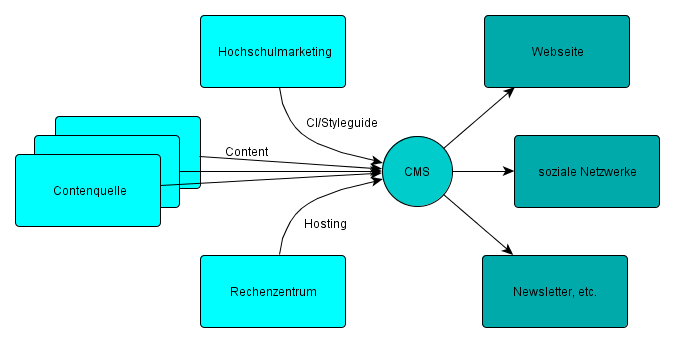
\includegraphics[width=15.501cm,height=7.853cm]{VorlaufigeSollSituationeblingsprafkeluebke-img/VorlaufigeSollSituationeblingsprafkeluebke-img001.png}
\caption[Verteilter Publishing Workflow]{Verteilter Publishing Workflow}

\end{figure}
\subsection{1.2 Internes Hochschulmarketing}
{\sffamily
Im Gegensatz zur Situation in einem Unternehmen genießen einzelne Fachbereiche und Personen in einer Hochschule einen
hohen Grad an Freiheit und Autonomie. Daher können in Arbeitsgruppen und Gremien beschlossene Prozesse und Software
nicht per Anordnung durchgesetzt werden, sondern müssen nach innen vermarktet werden, um akzeptiert zu
werden.Herausfordernd ist hier besonders die Heterogenität, da der technische und fachliche Hintergrund sich unter
Mitarbeitern und Fachbereichen erheblich unterscheiden dürften, etwa zwischen technischen und nichttechnischen
Fachbereichen.}

\subsection[1.2.1 Fokussierter Support]{1.2.1 Fokussierter Support}
{\sffamily
Eine Möglichkeit, Benutzer hin zu einer präferierten Lösung zu leiten ist diese in Präferenzen, Anleitungen und FAQs an
erster Stelle und in höherem Detailgrad zu präsentieren. Vielfach wird eine Voreinstellung einfach übernommen, und die
erste Lösung zu einer Fragestellung als Referenz angesehen.}

\subsection{1.2.2 Schulung}
{\sffamily
Eine weitere Maßnahme ist, Schulungen für die präferierten Lösungen anzubieten, die Vorteile der gefundenen Lösung
gegenüber anderen herausstellt. Optimal ist eine solche Lösung transparent, oder aber bietet Alleinstellungsmerkmale,
die eine Verwendung aus sich heraus attraktiv erscheinen lassen. Trotzdem kann es vorkommen, dass in Lern- und
Umstellungsphasen Lernkurven in der Benutzung absolviert werden müssen. Soll eine Lösung akzeptiert werden, dann muss
diese Lernkurve entsprechend begleitet werden.}

\subsection{1.2.3 Integration}
{\sffamily
Eine weitere starke, aber arbeitsintensive Maßnahme ist, die präferierte Lösung stark zu integrieren. Beispielsweise sei
die Erstellung von hochwertigen Dokumentvorlagen entsprechend der Corporate Identity für die präferierte
Textverarbeitung genannt.}

{\sffamily
Der Übergang zum fokussierten Support ist hier fließend. Wird die präferierte Lösung an das bestehende System angepasst,
so kann von Integration gesprochen werden, wird das System an eine präferierte Lösung angepasst, ist dies fokussierter
Support. Beides kann sehr gut gegenseitig ergänzend eingesetzt werden.}

\section{2 Support und Fortentwicklung}
{\sffamily
Support und Fortentwicklung hängen hier eng zusammen, da die Fortentwicklung hauptsächlich durch die im Support
gewonnenen Einsichten über Defizite in Prozessen vorangetrieben werden soll. So sollen Diskrepanzen zwischen
Erwartungen an das System und dessen tatsächlichen Fähigkeiten und Nutzung aufgedeckt und behoben werden.}

\subsection{2.1 Support}
{\sffamily
Supportleistung an einer kleinen Hochschule geschieht häufig direkt und unbürokratisch. Dieser ad-hoc-Ansatz bringt zwar
vielfach schnelle Hilfe, aber nur wenig zuverlässige Informationen über Prozessdefizite.}

\subsection{2.1.1 Zentrale Dokumentation}
{\sffamily
Die Vorteile dieser Art der Hilfeleistung sind für eine kleine Hochschule allerdings evident. Der Overhead mehr
reglementierter Supportsysteme würde einen unverhältnismäßigen Personalaufwand mit sich bringen, und Hilfeleistung
verzögern. Die Qualität des Supportprozesses selber würde damit sinken.}

{\sffamily
Notwendig zur besseren Identifizierung von Prozessdefiziten ist allerdings keine zentralisierte Supportleistung an sich,
sondern lediglich eine zentralisierte Dokumentation des geleisteten Supports.}

\begin{figure}
\centering
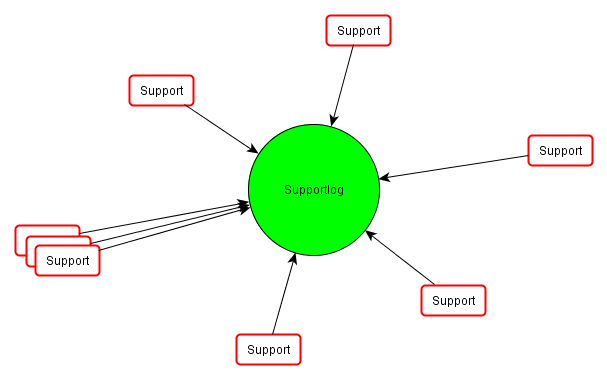
\includegraphics[width=15.501cm,height=9.678cm]{VorlaufigeSollSituationeblingsprafkeluebke-img/VorlaufigeSollSituationeblingsprafkeluebke-img002.png}
\caption[Unabhängige Supportleister dokumentieren in zentralem Log]{Unabhängige Supportleister dokumentieren in
zentralem Log}

\end{figure}
{\sffamily
Es ist dabei unerheblich, ob die Supportleister die Unterstützung als Kern ihrer Aufgabe leisten, oder ob es sich um
kollegiale Unterstützung bei einem Problem handelt. Gerade letztere Information aufzufangen ist wichtig, da diese sonst
nur eine sehr schwer einzuschätzende Größe bleibt.}

{\sffamily
Dieser Dokumentationsoverhead ist gering gegenüber dem Overhead eines stark reglementierten Supportsystems, erhält alle
Vorteile unbürokratischer, schneller Hilfeleistung und fängt zusätzlich Informationen über Art und Umfang gelisteten
Supports auf.}

\subsection{2.1.2 Knowledge Base}
{\sffamily
Aus dem Supportlog kann eine durchsuchbare Knowledge Base aufgebaut werden, die nicht nur die allgemeinen Fehlerquellen
und Schwierigkeiten von Software im Einsatz beleuchtet, sondern ganz speziell die an der Hochschule in dieser
Zusammenstellung einmalige Konfiguration.}

{\sffamily
Dadurch kann sehr viel schneller auf spezifische Fehlerszenarien reagiert werden, als dies mit allgemeinen Informationen
möglich ist.}

{\sffamily
Auch können aus dem Supportlog FAQs abgeleitet werden, die tatsächlich dem Wortsinn nach Listen häufig gestellter Fragen
und Antworten darstellen, und nicht was mehr oder minder begründet vermutet wird.}

{\sffamily
Auch zeigt sich in den Häufigkeiten bestimmter Probleme, wo spezielle Dokumentation und Hilfetexte notwendig sind, die
ebenfalls hinterlegt werden können.}

{\sffamily
Hierzu muss das Supportlog allerdings von einer geeigneten Stelle regelmäßig gesichtet werden.}

\subsection{2.2 Fortentwicklung}
{\sffamily
Eine Konzeption kann nur aktuelle Trends und Entwicklungen berücksichtigen. Es ist schwierig vorauszuschauen, was die
Zukunft danach bringen wird, welche Trends mehr oder weniger wichtig sind, und welche Trends darauf folgen werden.
Allerdings ist es keine Frage, dass eine Hochschule länger Bestand hat, und es damit sinnvoll ist, Prozesse zu
hinterlegen, die neue Trends und Entwicklungen zwar nicht vorwegnehmen, aber deren zeitnahe Entdeckung und Integration
ermöglichen.}

{\sffamily
Auch zeigt sich in der Praxis, dass unvorhergesehene Bedingungen und Ereignisse theoretisch gut ausgearbeitete Prozesse
übermäßig blockieren, und eine Anpassung geschehen muss.}

\subsection{2.2.1 Feedback}
{\sffamily
Hierzu muss an jedem Punkt des Gesamtsystems dem Benutzer möglich sein, Feedback zu geben. Mehr noch muss gerade bei
neuen oder überarbeiteten Prozessen dieses Feedback eingefordert werden, um die Qualität des neuen Prozesses oder Tools
einschätzen zu können.}

{\sffamily
Das Feedback gelangt an die zuständige Stelle, muss aber auch zentral gesammelt werden, ähnlich wie das Supportlog.
Diese Sammlung wird zentral ausgewertet, um verdeckte, verteilte Probleme aufzudecken, die sich in Feedback an
unterschiedliche Stellen verbergen können.}

{\sffamily
Auf die Auswertung muss wo sich Probleme zeigen, eine Information der zuständigen Stelle folgen, damit eine Verbesserung
erarbeitet werden kann. Entsprechend ist die zuständige Stelle berechtigt, ein Meeting einzuberufen, damit ihre
Eingaben nicht einfach verloren gehen können, sondern zwangsläufig mindestens einmal besprochen werden.}

\subsection{2.2.2 Innovationseingabe}
{\sffamily
In den Feedbackprozess eingebettet muss die Möglichkeit für jede Person sein, Innovationen aus beliebiger Quelle zu
beschreiben, so dass Entwicklungen nicht erst von bestimmter Stelle wahrgenommen werden müssen, um erwägt zu werden.
Damit kann von beliebiger Stelle aus eine Verbesserung zur Diskussion gebracht werden.}

{\sffamily
Damit diese Möglichkeit von Benutzern angenommen wird, muss auf Eingaben angemessen schnell reagiert werden. Um eine
ernsthafte Reaktion zu gewährleisten, müssen diese Vorschläge auch diskutiert worden sein.}

\subsection[2.2.3 Erfahrungsgetriebene Fortentwicklung]{2.2.3 Erfahrungsgetriebene Fortentwicklung}
{\sffamily
Aus den Erkenntnissen über Schwachstellen aus dem Supportlog, den Benutzerberichten und -bewertungen aus dem Feedbacklog
und den Innovationseingaben können nicht nur Schwachstellen und Fehler in Prozessen identifiziert werden, sondern auch
Trends in der Benutzung des Systems erkannt. Da Support und Feedback andauernde Prozesse sind, ergibt sich daraus ein
selbstregulierendes System, das, wenn die Messgrößen Supportlog und Feedbacklog angemessen berücksichtigt werden,
evolutionär verbessert.}



\begin{figure}
\centering
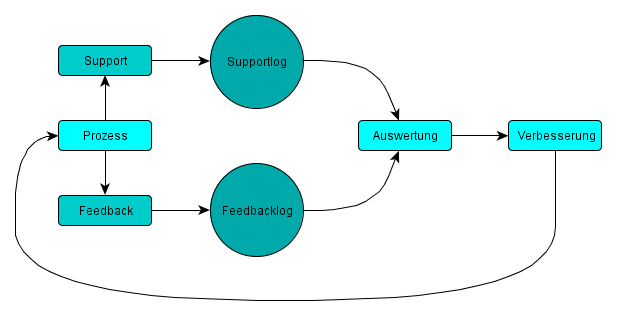
\includegraphics[width=15.501cm,height=7.913cm]{VorlaufigeSollSituationeblingsprafkeluebke-img/VorlaufigeSollSituationeblingsprafkeluebke-img003.png}
\caption[Zyklus der Verbesserung eines Prozesses]{Zyklus der Verbesserung eines Prozesses}

\end{figure}
\clearpage\section{Hard- und Software}
{\sffamily
Zur Integration eines hochschulweiten Informationsmanagements können bezüglich der IT mehrere Ansätze gefahren werden.}

{\sffamily
Zum einen kann eine ganzheitliche integrierte Lösung verwendet werden. Die Universität Hamburg hat einen vollständigen
Neuanfang bezüglich der Campussoftware gewagt mit der integrierten Gesamtlösung „CampusNet“ der Datenlotsen
Informationssysteme GmbH. Dies resultierte aus der Zusammenlegung mehrerer Fachbereiche zu einzelnen Fakultäten. Die
verschiedenen Teillösungen waren größtenteils inkompatibel oder aufgrund von Eigenentwicklung schwer
wartbar.\footnote{DINI: Personalisierte Webportale für Hochschulen}}

{\sffamily
Laut Günter Müller, Leiter des Rechenzentrums, existieren an der Hochschule Emden Leer derart verschiedene Teillösungen
nicht. Auch würden sich Eigenentwicklungen auf vernachlässigbare Systeme beschränken. Software würde grundsätzlich für
die gesamte Hochschule eingesetzt.\footnote{Interview}}

{\sffamily
Der Einsatz einer integrierten Gesamtlösung zur Beseitigung von Inkompatibilitäten und schwer wartbaren
Eigenentwicklungen kann somit keine Argumentationsgrundlage sein.}

{\sffamily
Des Weiteren reicht die bisherige Analyse nicht aus, um einen vollständigen Anforderungskatalog zu bilden, auf dessen
Grundlage eine integrierte Gesamtlösung gefunden werden kann. }

{\sffamily
Stattdessen wird auf eine flexible Lösung gesetzt, welche den Einsatz einzelner Fachanwendungen zur Lösung bestimmter
Probleme vorsieht. Personelle und finanzielle Ressourcen sind dadurch flexibler einsetzbar, auf veränderte
Anforderungen an eine Lösung kann flexibler reagiert werden und die Abhängigkeit von einem Anbieter für alle
Anwendungen wird aufgelöst.}

\subsection{Kernanforderungen}
{\sffamily
Bei Core-Systemen wird weiterhin auf Appliance Lösungen gesetzt. Das minimiert}

{\sffamily
\ Fehlerpotenzial und den operativen Betrieb.\footnote{Interview}}

{\sffamily
Softwaresysteme laufen auf virtuellen Maschinen. Die bessere Hardwareauslastung und Möglichkeit der automatisierten
Administration kann finanzielle und personelle Ressourcen sparen.\footnote{Baun, Kunze, Ludwig: Servervirtualisierung}
Die Systeme sind weniger abhängig von der Hardware, was dessen Austausch erleichtert. Netzwerkanbindung, Rechenleistung
und Speicherkapazität sind somit flexibler an sich verändernde Anforderungen anpassbar.}

{\sffamily
Die eingesetzte Software soll in die Systemlandschaft integrierbar, lösungsorientiert und möglichst barrierefrei, sowie
systemunabhängig sein. Dies unterstützt auch den Ansatz der Freiheit in Forschung und Lehre.}

{\sffamily
Die Systemunabhängigkeit kann durch Webanwendungen im Sinne des Ansatzes Software as a Service (SaaS) erreicht werden.
Um möglichst alle gängigen Browser und Endgeräte zu unterstützen, sollten die Anwendungen den Standards des World Wide
Web Consortiums (W3C) gerecht werden und sofern möglich dem Ansatz responsive design gerecht werden. Dadurch kann auch
dem Trend bring your own device Rechnung getragen werden.}

\subsection{Bereichsübergreifende Basissysteme}
{\sffamily
In den Bereichen Forschung, Lehre und Verwaltung fallen informationstechnologische Aufgaben an, für die eine zentrale
IT-gestützte Lösung geschaffen werden kann. Das verringert redundante Daten und Systeme sowie administrative Aufwände.
Im folgenden werden Lösungen für einzelne Aspekte des Informationsmanagements aus IT-Sicht vorgestellt, die in allen
drei Bereichen genutzt werden können. Weiterhin dienen sie teilweise als Grundlage für spezialisierte Systeme.}

\subsubsection{Identity Management}
{\sffamily
Um die Anzahl an verschiedenen Accounts zu minimieren, sollten die Benutzer zentral gepflegt werden. Dies kann in einem
Verzeichnisdienst wie dem bereits eingeführten Active Directory geschehen. Die Authentifizierung an einem System}

{\sffamily
findet dann nicht am System selbst statt, sondern mit Hilfe des Verzeichnisdienstes. Der Anwender muss sich nur einen
Account zzgl. Kennwort merken, um sich an verschiedenen Systemen anzumelden. Weiterhin gilt eine Aktualisierung von
Informationen global, wodurch Inkonsistenzen aufgelöst werden.}

{\sffamily
Zuzüglich zum zentralen Verzeichnisdienst ist auch ein SingleSignOn (SSO) Mechanismus empfehlenswert\footnote{Zahn: vom
ITS zum IT-Management}, wie es an der Universität Augsburg durch das System Webauth umgesetzt ist. Für das
Lernraumsystem moodle gibt es bereits ein SSO Plugin\footnote{http://sourceforge.net/projects/moodleldapsso}. Alle
weiteren Websysteme sollen auf SSO umgestellt werden, um dem Benutzer eine möglichst integrierte Landschaft zu bieten.
Weiterhin sollte jedes System aus Sicherheitsgründen insofern angepasst werden, dass auch ein SingleSignOff möglich
ist. Die zentrale Abmeldung soll gewährleisten, dass die Benutzenden auf allen Systemen, auf denen sie sich bewegt
haben, abgemeldet sind.}

{\sffamily
Die Benutzerdatenpflege sollte auf den einzelnen Systemen ausgeschaltet sein und ausschließlich über ein zentrales
Formular geschehen. So wird ein konsistenter Datenbestand gesichert. Insofern die Informationen in anderen Systemen
benötigt werden, müssen diese vom zentralen System automatisiert und über gesicherte Verbindungen verteilt werden. Ein
weiterer Vorteil ist, dass die Informationen, da zentral gesammelt, auch zentral ausgewertet werden können.}

{\sffamily
So ist es möglich diese zentralen persönlichen Informationen mit Informationen anderer Art aus anderen Systemen
anzureichern und weiterzuverwenden. So können automatisierte Reports über Forschungsprojekte erstellt werden,
Expertisen zu bestimmten Themen identifiziert werden oder für die Verwaltung Verknüpfungen von Personen zu
verwaltungstechnischen Aufgaben. Die Umsetzung ist dabei individuell an die Gegebenheiten und Informationsbedarfe der
Hochschule anzupassen.\footnote{Grote, Mersch: Design des Identitätsmanagements} Dementsprechend wird die technische
Lösung eine Individuallösung werden.}


\bigskip

\clearpage\subsubsection{Geschäftsprozesse}
{\sffamily
Neben der Forschung gibt es an Hochschulen gerade im Verwaltungsbereich viele Geschäftsprozesse, die in der Regel immer
gleich ablaufen. Problem ist, dass Personen unterschiedlichster Bereiche involviert sind und die Prozesse nicht
ausreichend definiert sind.\footnote{Becker: Prozessorientierte Verwaltungsmodernisierung an Hochschulen}}

{\sffamily
Die Modellierung der Prozesse sollte im ersten Schritt auf abstraktem Niveau stattfinden. Dies erleichtert den Einstieg
und macht Verbesserungspotenziale sichtbarer. In der WWU Münster wurde dafür die PICTURE Methode verwendet.}

{\sffamily
Im zweiten Schritt kann der ggf. angepasste Prozess konkretisiert und in Form des Industriestandards Business Process
Model Notation (BPMN) festgehalten werden. Ein Client-Tool zur Erstellung von BPMN ist das Activiti BPMN 2.0 Eclipse
Plugin.\footnote{http://docs.codehaus.org/display/ACT/Activiti+BPMN+2.0+Eclipse+Plugin}}

{\sffamily
Mit Hilfe der zentralen Business Process Management (BPM) Platform activiti können die Prozesse aktiv den Workflow
verbessern, Konsistenz wahren und zeitliche Ressourcen sparen. \ Die Plattform ermöglicht REST Anfragen, wodurch die
Prozessinformationen auch in andere Applikation integriert werden können. Der Activiti Explorer ermöglicht den voll
funktionalen Zugriff via Weboberfläche. Somit wird der Kernanforderungen SaaS Rechnung getragen. Weiterhin ist Activiti
Open Source und somit ausbau- und anpassungsfähig.\footnote{http://activiti.org/index.html}}

{\sffamily
Durch activiti wird es möglich sein die Automatisierung von einzelnen Prozessen Stück für Stück voranzutreiben. Einzelne
Teile des Workflows können automatisiert Scripte starten, E-Mails verschicken und ähnliches und somit stückweise die
manuelle Bearbeitung reduzieren. Außerdem können Serviceanfragen damit zentralisiert verwaltet werden. Durch Definition
von Feldern für einzelne Prozessschritte können vorab benötigte Informationen festgelegt werden, sodass Nachfragen
vermieden werden.}

\clearpage\subsubsection{Content Management}
{\sffamily
Um den wachsenden Anforderungen in Bezug auf Content Management genüge zu tun wurde an der WWU Münster das Enterprise
Content Management System alfresco eingeführt.}

{\sffamily
Auch an einer kleinen Hochschule kann ein solches System eingesetzt werden. Alfresco bietet diverse Vorteile. Die für
dieses Konzept Relevanten werden hier kurz aufgelistet\footnote{Tröger, Lorenz, Klötgen, Przibytzin: Das digitale
wissenschaftliche Informationssystem der WWU}:}

\liststyleLi
\begin{itemize}
\item {\sffamily
Unterstützung für mobile Endgeräte}
\item {\sffamily
Anpassungs- und ausbaufähig}
\item {\sffamily
diverse Zugriffsmöglichkeiten zur Nutzung innerhalb bekannter Standardanwendungen}
\item {\sffamily
Publikation in soziale Netzwerke}
\item {\sffamily
Unterstützung verschiedener Standardschnittstellen}
\item {\sffamily
Activiti Workflow Engine}
\item {\sffamily
Metadaten}
\end{itemize}
{\sffamily
Alfresco bietet damit die ideale Grundlage verschiedene Informationen zu verwalten sowie die Unterstützung des
vollständigen Dokumenten-Lifecycles - von der Erstellung über die Bereitstellung bis zur Archivierung. Die Anbindung
der Dokumente ist dynamisch und durch die zahlreichen Standards ideal integrierbar. So kann ein an verschiedenen Orten
auf verschiedene Arten bereitgestelltes Dokument an einer Stelle aktualisiert werden wodurch an allen Zugriffsstellen
die aktuellste Version bereitgestellt wird. Dennoch ist das System flexibel genug auch bestimmte Versionen eines
Dokuments bereitzustellen. Dank der integrierten Versionierung entfällt außerdem der aufwendige
Wiederherstellungsprozess. Dank der Möglichkeit Metadaten anzugeben, wird der Weg für eine brauchbare Dokumentensuche
geebnet.}

\clearpage\subsection{Spezialsysteme}
{\sffamily
Unter Spezialsystemen sind hier Softwarelösungen zu verstehen, die bei speziellen Aufgaben im Hochschulalltag
unterstützen sollen.}

\subsubsection{Verwaltungssoftware}
{\sffamily
Software, die speziell in der Verwaltung genutzt wird, ist in dieser Ausarbeitung ausgenommen, da die Anforderungen sehr
speziell sein können und die Wissensbasis innerhalb dieser Ausarbeitung nicht ausreicht, um eine Empfehlung zu geben.}

{\sffamily
Erwähnt werden sollte dennoch, dass die Universität Karlsruhe erfolgreich Schnittstellen zu den HIS-Systemen integriert
hat.\footnote{DINI: Personalisierte Webportale für Hochschulen}}

{\sffamily
Da dieses Konzept auf einem ähnlich flexiblen Ansatz basiert, besteht die Möglichkeit, dass auch Verwaltungssoftware
integriert werden kann, wenn sie die genannten Kernanforderungen erfüllt.}

\subsubsection{Lernplatform}
{\sffamily
Die Hochschule setzt bereits erfolgreich und in vielen Bereichen das System moodle ein. Die Nutzung der Funktionen
variiert dabei zwischen den einzelnen Fachbereichen.}

{\sffamily
So lange moodle die Anforderungen der Hochschule an eine Lernplattform erfüllt, besteht kein Grund das System
auszutauschen.}

{\sffamily
Neben den bereits genutzten Standardfunktionen ist moodle ausbaufähig.}

{\sffamily
Beim Aufruf von moodle soll die Authentifizierung durch einen SSO Mechanismus geschehen. Hat sich ein Benutzer bereits
an einem anderen System authentifiziert, ist dieser beim Aufruf sofort angemeldet. Integriert werden sollte auch der
SingleSignOff Mechanismus.}

{\sffamily
Statt der Stammdatenänderung via moodle wird auf ein zentrales Formular weitergeleitet, um persönliche Informationen
zentral und damit konsistent zu halten.}

{\sffamily
Die in den Kursen zur Verfügung gestellten Dateien jeglicher Art werden in alfresco gepflegt und von moodle angebunden.
Die entsprechenden Schnittstellen}

und Plugins müssen nicht neu entwickelt werden. Vorteil ist, dass die Dokumente in alfresco verwaltet werden. In moodle
kann dann eine bestimmte Version oder die jeweils aktuellste referenziert werden. Bei den Dokumenten kann es sich um
Textdokumente, Audio oder auch Videofiles handeln. Durch alfrescos Unterstützung für mobile Endgeräte wird so den
Zugreifenden auch die Möglichkeit gegeben ein Dokument auf den verschiedensten Endgeräten anzuzeigen.

{\sffamily
Dank alfresco können Dokumente nicht nur innerhalb moodle via Weboberfläche aufgerufen werden, sondern auch bequem via
Filesystem. Eine Datei kann somit auf verschiedene Art und Weise abgerufen werden – je nach dem welchen Weg der
Anwender für den aktuell praktikabelsten hält.}

\subsubsection{Publikationen}
{\sffamily
Um Wissenschaftler bei der Publikation von Zeitschriften zu unterstützen setzt die WWU Münster auf die Plattform Open
Journal System (OJS). Es bietet die Möglichkeit elektronische Zeitschriften zu verwalten und den gesamten
Publikationsworkflow abzubilden\footnote{Tröger, Lorenz, Klötgen, Przibytzin: Das digitale wissenschaftliche
Informationssystem der WWU}.}

{\sffamily
Grundsätzlich sollte auch ein Workflow in activiti implementiert werden, der bei der Publikation unterstützt. So können
wichtige Metadaten aufgenommen und an relevante Systeme weitergegeben werden. Ändern sich Systeme oder kommen neue
hinzu, müssen sich Wissenschaftler nicht umgewöhnen, sondern nutzen weiterhin den in activiti hinterlegten, für die
neuen Systeme jedoch angepassten, Prozess. Dadurch besteht auch die Möglichkeit ein publiziertes Dokument zusätzlich in
alfresco abzulegen, wenn ein Anwendungsfall dies benötigt.}

{\sffamily
OJS bietet die Möglichkeit der Authentifizierung via Single Sign On. Dies geschieht via
Shibboleth.\footnote{https://pkp.sfu.ca/wiki/index.php?title=Setting\_up\_authentication} Neben der Konfiguration von
Single Sign On sollte auch hier den Benutzenden die Möglichkeit des Single Sign Off gegeben werden.}

\clearpage\subsubsection{Evaluation}
{\sffamily
Wie auch die Universität Münster\footnote{https://www.wiwi.uni-muenster.de/fakultaet/de/studium/lehrevaluation} und die
TU Dortmund\footnote{https://www.itmc.uni-dortmund.de/dienste/e-learning/umfragewerkzeuge.html} setzt die Hochschule
Emden Leer bereits die Software EvaSys zu Evaluationszwecken ein. Sie ist webbasiert und entspricht damit dem Software
as a Service Gedanken.}

{\sffamily
Seit Version 5 unterstützt EvaSys auch die SingleSignOn
Authentifizierung\footnote{http://www.ku.de/fileadmin/190304/Feature\_Function\_Benefit\_EvaSys\_V5.0\_DE.pdf}, welche
auch an der Hochschule Emden Leer eingesetzt werden soll.}

\subsubsection{Campus Portal}
{\sffamily
Ein Campus Portal dient als zentrale Anlaufstelle für alle Hochschulangehörigen und ist ein personalisiertes Webportal.
Es soll die Verwaltung persönlicher Daten ermöglichen, eine Übersicht über informationstechnische Funktionen inklusive
Weiterleitung zum entsprechenden System integrieren, sowie aktuell relevante Informationen in Form einer Agenda
anzeigen.}

{\sffamily
Unter den informationstechnischen Funktionen sind alle Werkzeuge und Systeme zu verstehen, die einem bestimmten Zweck
dienen. Eine Selbstimplementierung für die bereitzustellenden Funktionen soll dabei vermieden werden. Stattdessen soll,
wie in den Kernanforderungen aufgenommen, auf existierende Systeme gesetzt werden, sofern dies möglich ist. Beim Campus
Portal werden die Kernanforderungen an diese Systeme, nämlich integrierbar und systemabhängig (SaaS) zu sein, nun
deutlich.}

{\sffamily
Ein solches Campus Portal ist vor allem der Informationsübersicht dienlich. Durch personalisierte und dynamisch
generierte Inhalte gewinnen die Benutzenden einen Überblick über die Informationen, die sonst in verschiedenen Systemen
verteilt sind.}

{\sffamily
Die Integration der Systeme kann schrittweise erfolgen, sollte jedoch zur Akzeptanzgewinnung bei Veröffentlichung eine
gewisse Menge externer Systeme integrieren. Die Universität Karlsruhe hat im ersten Schritt das
Verantstaltungsmanagement und die Prüfungsverwaltung der Software-Systeme}


\bigskip

der HIS GmbH in das Portal integriert.

{\sffamily
Orientiert am Anforderungskatalog der WWU Münster an ein solches Portal\footnote{Vogl, Tröger, Schwartze: Fortschritte
des integrierten Informationsmanagements and Hochschulen} und unter der Voraussetzung, dass die in diesem Konzept
genannten Systeme umgesetzt werden, kann ein zukünftiges CampusPortal folgende Informationen konsolidieren.}

\liststyleLii
\begin{itemize}
\item {\sffamily
Kalender}

\begin{itemize}
\item {\sffamily
Abonnement-Prinzip}
\item {\sffamily
Detailinformationen zum Beispiel Kontoinformationen für Rückmeldungsgebühren}
\item {\sffamily
Agenda aus moodle}
\end{itemize}
\item {\sffamily
Referenz zu gewählten Kursen (moodle)}
\item {\sffamily
Referenz zum E-Mail Portal (Outlook Web App)}
\item {\sffamily
Suchmaschine}
\item {\sffamily
offene Tasks im BPM System}
\item {\sffamily
Start möglicher Tasks im BPM System (zum Beispiel ein Workflow für die Publikation)}
\item {\sffamily
offene Evaluationen}
\end{itemize}
{\sffamily
Unter der Voraussetzung, dass auch andere Hochschulsysteme integrierbar sind, können folgende Punkte aus dem
Anforderungskatalog der WWU Münster zusätzlich im Campus Portal integriert werden:}

{\sffamily
Stundenplan}
{\sffamily
Vorlesungsverzeichnis inkl. Details}
{\sffamily
Leistungsübersicht}
{\sffamily
Hochschulleben}

{\sffamily
Mensapläne}
{\sffamily
Hochschulsport}
{\sffamily
Veranstaltungen}
{\sffamily
Einführung}
\clearpage{\sffamily
\newline
Alternativ dazu kann auch das Konzept eines Hilfesystems integriert werden, das via Sprechblasen Hilfestellungen oder
Informationen anzeigt zur Funktion auf der sich der Mauszeiger gerade befindet}
{\sffamily
Die technische Struktur kann analog zu der des Portals myWWU der Universität Münster aufgebaut sein.}

\subsubsection[Integrierte Gesamtsuche]{Integrierte Gesamtsuche}
\begin{figure}
\centering
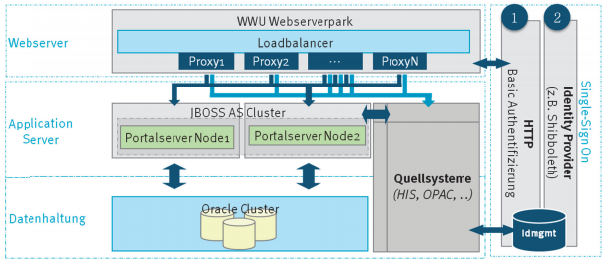
\includegraphics[width=15.501cm,height=6.675cm]{VorlaufigeSollSituationeblingsprafkeluebke-img/VorlaufigeSollSituationeblingsprafkeluebke-img004.png}
\caption[technische Struktur des Portals myWWU der Universität Münster]{technische Struktur des Portals myWWU der
Universität Münster}

\end{figure}
{\sffamily
Wissenschaftliche Informationen sind häufig in verschiedenen Systemen angesiedelt. Durch die Einführung eines Systems
zur integrierten Gesamtsuche wird die Suche an zentraler Stelle ausgeführt. Einzelne Systeme werden beim Suchen nicht
vergessen. Die Integration neuer Systeme erleichtert die Kommunikation derer Integration in das wissenschaftliche
Umfeld. Die WWU Münster nutzt dafür einen „Suchmaschinen-basierte[n] Ansatz auf Basis der Software Primo von der Firma
Ex Libris“.\footnote{Vogl, Tröger, Schwartze: Fortschritte des integrierten Informationsmanagements and Hochschulen}}
{\sffamily
Dafür nötig ist eine Normalisierung der Datenformate interner und externer Quellen, welche „insbesondere auf der
Detailebene […] aufwändige Anpassungen und Eigenentwicklungen notwendig“ machen.}
\clearpage
\bigskip
{\sffamily
Quellsysteme ausgehend von diesem Konzept können sein:}

\liststyleLiii
\begin{itemize}
\item {\sffamily
alfresco}
\item {\sffamily
Identity Management System}
\item {\sffamily
ForschungsDB Niedersachsen}
\item {\sffamily
moodle}
\item {\sffamily
Open Journal System}
\item {\sffamily
Hochschulexterne Informationssysteme wie zum Beispiel video2brain}
\item {\sffamily
ggf. Bibliothekssuche}
\end{itemize}
{\sffamily
Wichtig ist neben korrekten und vollständigen Ergebnissen auch die Benutzbarkeit. Bekannte Funktionalitäten aus anderen
Suchmaschinen, wie Gruppierungen, sollten integriert sein, wie auch eine übersichtliche und funktionale
Benutzeroberfläche.}

\subsubsection{Ausblick bei Integration der Bibliothek}
{\sffamily
Die Best Practices zeigen, dass auch die Bibliotheken der Hochschulen und Universitäten bei
Informationsmanagement-Projekten integriert werden. Die dort vorhandenen Informationen werden vor allem für Forschung
und Lehre genutzt, welches die Kernaufgaben von Hochschulen sind.}

{\sffamily
Neben der Anbindung der Bibliothekssuche in die integrierte Gesamtsuche kann auch ein Digitalisierungssystem für
archivierte Zeitschriften und Bücher zur Aufwertung der gesuchten Informationen beitragen. Die WWU Münster setzt dafür
das vor Ort frei verfügbare Scanner zuzüglich der Software scantoweb ein.}

\clearpage{\sffamily\bfseries
Abwägung des Einsatzes eines Informationsmanagers an der Hochschule Emden}

{\sffamily
Das Soll-Konzept analysiert die Ist-Situation um festzustellen, ob es generell einer Verbesserung des
Informationsmanagements bedarf und wo diese anzusetzen sind oder ob noch kein Informationsmanagement besteht und
aufgebaut werden muss. Dazu sind verschiedene Aspekte zu beleuchten. Neben der Anforderung des Marketings und neben den
\ technischen Neuerungen und Umsetzungen ist zu klären, wer die strategische und operative Führung übernehmen soll. }

\textsf{Im klassischen Informationsmanagement ist dies die Aufgabe eines Chief Information Officers. Der
Informationsmanager dient dabei als zentrale Schnittstelle zwischen technischen, organisatorischen und wirtschaftlichen
Teilbereichen und dient dort als sogenannter Mittler und untersucht dafür die Informations- und Kommunikationstechniken
in allen unterschiedlichen Bereichen um diese sinnvoll einzusetzen.}\footnote{\ \{Krcmar 2015 \#1, S. 86\}}

{\centering

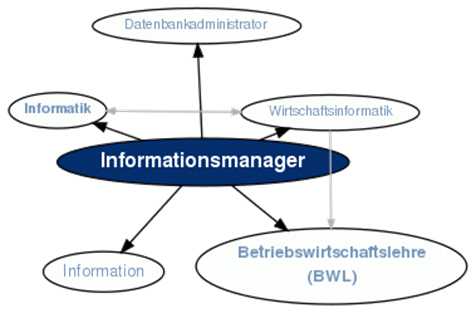
\includegraphics[width=12.139cm,height=7.982cm]{VorlaufigeSollSituationeblingsprafkeluebke-img/VorlaufigeSollSituationeblingsprafkeluebke-img005.jpg}
\newline
\textsf{Abb. 1}\footnote{\ \{Definition \ Informationsmanager \ {\textbar} \#5\}\par }
\par}

\clearpage
\bigskip

{\sffamily\bfseries
Analyse des Ist-Zustandes}

\textsf{Bezug nehmend auf die Abb. 2 und der festgestellten Ist-Analyse ist festzuhalten, dass der Hochschule Emden kein
Informationsmanagement im klassischen Sinne zugrunde liegt, sondern ein zentrales Informationssystem. Es werden
verschiedene Dienste und Möglichkeiten wie Moodle, Eduroam zur Verfügung gestellt \ und in Anspruch genommen. Es gibt
keine Verwaltung sondern verschiedene Bereiche die unterteilt sind in Arbeitsgruppen, Abteilungen sowie Rechenstelle
und Pressestelle. Weiterhin beinhaltet das Informationssystem verschiedene Prozesse zum Datenaustausch, bzw. Datenfluss
und Backuptransfer \ aus verschiedenen Systemen.}\footnote{\ \{Ist-Situation \#8\}}\textstyleFootnoteSymbol{\textsf{
}}\textsf{Die Nutzung des gegenwärtigen Informationssystems wird unterschiedlich stark genutzt oder ausgelastet. }

\textsf{Von den zentralen Einrichtungen nehmen das Hochschulrechenzentrum und die Bibliothek einen wichtigen Platz in
der Hochschule ein. Das Hochschulrechenzentrum übernimmt derweil viele Aufgaben der Informationsverwaltung und Planung.
Doch nicht nur da werden Informationen gesammelt und \ ausgewertet. Die Hochschule in Emden definiert eine ganze Reihe
von Arbeitsgruppen, beispielsweise die Arbeitsgruppe Zahlen, Daten, Fakten, die Kennzahlen der Hochschule und der
einzelnen Fachbereiche sammelt und diese auswertet.}\footnote{\ \{Ist-Situation \#8\}}\textsf{ Aktuell besteht keine
Vernetzung verschiedener Intranetzsysteme zwischen verschiedenen Hochschulen.
}\textstyleAbsatzStandardschriftart{\textsf{\textit{\textcolor[rgb]{0.8509804,0.8509804,0.8509804}{Der aktuelle
Austausch erfolgt über Foren, die …}}}}

\textstyleAbsatzStandardschriftart{\textsf{\textbf{\textcolor[rgb]{0.8,0.8,0.8}{weitere Ausführungen folgen noch...}}}}



\begin{figure}
\centering
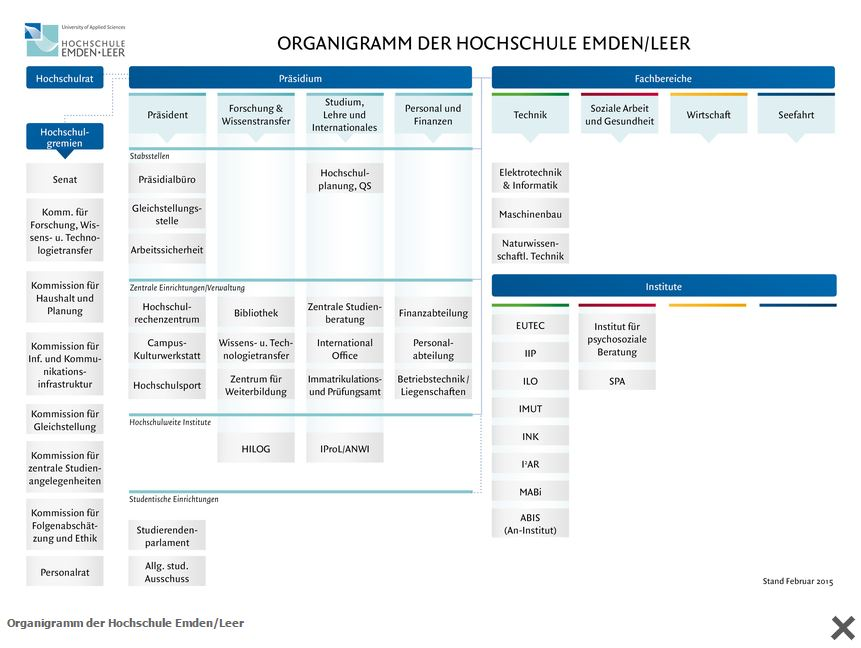
\includegraphics[width=17.731cm,height=12.446cm]{VorlaufigeSollSituationeblingsprafkeluebke-img/VorlaufigeSollSituationeblingsprafkeluebke-img006.jpg}
\end{figure}

\bigskip


\bigskip


\bigskip


\bigskip


\bigskip

\newline
\textstyleAbsatzStandardschriftart{\textsf{\textbf{Abb. 2}}}\footnote{\ \{Emden/Leer 2015 \#7\}}


\bigskip

\clearpage
\bigskip

{\sffamily\bfseries
Analyse des zu erwartenden Soll-Zustandes}


\bigskip

{\sffamily
Nach Betrachtung der Best-Practice Beispiele anderer Hochschulen, lässt sich erkennen, dass jede Hochschule und auch
Universität den Umgang des Informationsmanagements anders angeht. So spielen verschiedene Faktoren eine Rolle, die an
jeder Hochschule unterschiedlich ausgelegt sind. Ein \ Vergleich der betrachteten Hochschulen mit der Hochschule Emden
zeigt, dass Emden eine wesentlich kleinere Hochschule ist und somit andere Ansprüche und nicht so komplexe Strukturen
besitzt, als beispielsweise die WWW Münster, die über 40.000 Studierende pflegt. Trotz unterschiedlich integrierter
Möglichkeiten zur Umsetzung des jeweiligen Informationsmanagements, gibt es doch Bereiche die gleich oder relativ
ähnlich sind. So sind Bibliotheken, Gremien, Ausschüsse, ebenso wie Fachbereiche und auch das Präsidium Teil einer
jeden Hochschule oder Universität. }

{\sffamily
\newline
Es \ ist zu schauen wo sich das Informationsmanagement ansetzen lässt um mehrere Bereiche und Bestandteile untereinander
zu verbinden. Fakt ist, dass es in Emden bereits Arbeitsgruppen gibt, die bestimmte Informationen gewinnen und filtern.
So wäre der Aufbau einer neuen Struktur eine Möglichkeit zur Verbesserung des Informationsaustausches.}


\bigskip


\bigskip

{\sffamily\itshape\color[rgb]{0.8509804,0.8509804,0.8509804}
MIRO Projekt vergleichen?\newline
Möglichkeiten Bereiche übernehmen?\newline
Überhaupt sinnvoll?}

{\itshape\color[rgb]{0.8509804,0.8509804,0.8509804}
\textstyleFootnoteSymbol{\textsf{\textbf{IKM Service für Emden vergleichen \newline
Mögliche Bereiche übernehmen?\newline
Überhaupt sinnvoll?}}}}

{\itshape\color[rgb]{0.8509804,0.8509804,0.8509804}
\textstyleFootnoteSymbol{\textsf{\textbf{→ aufnehmen }}}}

\clearpage
\bigskip

{\sffamily\bfseries
Soll-Möglichkeit ...}

[Warning: Draw object ignored]


\bigskip


\bigskip


\bigskip

\clearpage
\bigskip

{\sffamily\bfseries
Zu erwartende Kosten}


\bigskip

{\sffamily
Stichpunkte Überlegungen}

{\sffamily
Personalkosten durch höheren Aufwand}

{\sffamily
Weiterbildung}

{\sffamily
Vernetzung des Hochschulverbundes (einmalige Kosten bzw. weiterführende Kosten)}

{\sffamily
Budgetierung}

{\sffamily
Bessere Optimierungen des Haushaltes zur Optimierung des Informationsmanagements}

{\itshape\color[rgb]{0.8509804,0.8509804,0.8509804}
\textstyleAbsatzStandardschriftart{\textsf{…}}}

\clearpage
\bigskip

\textstyleAbsatzStandardschriftart{\textsf{\textbf{Prognose und zu erwartender Verlauf/ Fazit}}}


\bigskip

{\sffamily
Folgt noch}


\bigskip
\end{document}
